% -----------------------------------------------
% Template for SMC 2020
% adapted from previous SMC paper templates
% -----------------------------------------------

\documentclass{article}
\usepackage{smc2020}
\usepackage{times}
\usepackage{ifpdf}
\usepackage[english]{babel}
\usepackage{cite}
\usepackage{amsmath}

%%%%%%%%%%%%%%%%%%%%%%%% Some useful packages %%%%%%%%%%%%%%%%%%%%%%%%%%%%%%%
%%%%%%%%%%%%%%%%%%%%%%%% See related documentation %%%%%%%%%%%%%%%%%%%%%%%%%%
%\usepackage{amsmath} % popular packages from Am. Math. Soc. Please use the 
%\usepackage{amssymb} % related math environments (split, subequation, cases,
%\usepackage{amsfonts}% multline, etc.)
%\usepackage{bm}      % Bold Math package, defines the command \bf{}
%\usepackage{paralist}% extended list environments
%%subfig.sty is the modern replacement for subfigure.sty. However, subfig.sty 
%%requires and automatically loads caption.sty which overrides class handling 
%%of captions. To prevent this problem, preload caption.sty with caption=false 
%\usepackage[caption=false]{caption}
%\usepackage[font=footnotesize]{subfig}


%user defined variables
\def\papertitle{Resurrecting the Tromba Marina: the impact of a friction model on the interaction with a virtual instrument}
\def\firstauthor{First author}
\def\secondauthor{Second author}
\def\thirdauthor{Third author}

% adds the automatic
% Saves a lot of output space in PDF... after conversion with the distiller
% Delete if you cannot get PS fonts working on your system.

% pdf-tex settings: detect automatically if run by latex or pdflatex
\newif\ifpdf
\ifx\pdfoutput\relax
\else
   \ifcase\pdfoutput
      \pdffalse
   \else
      \pdftrue
\fi

\ifpdf % compiling with pdflatex
  \usepackage[pdftex,
    pdftitle={\papertitle},
    pdfauthor={\firstauthor, \secondauthor, \thirdauthor},
    bookmarksnumbered, % use section numbers with bookmarks
    pdfstartview=XYZ % start with zoom=100% instead of full screen; 
                     % especially useful if working with a big screen :-)
   ]{hyperref}
  %\pdfcompresslevel=9

  \usepackage[pdftex]{graphicx}
  % declare the path(s) where your graphic files are and their extensions so 
  %you won't have to specify these with every instance of \includegraphics
  \graphicspath{{./figures/}}
  \DeclareGraphicsExtensions{.pdf,.jpeg,.png}

  \usepackage[figure,table]{hypcap}

\else % compiling with latex
  \usepackage[dvips,
    bookmarksnumbered, % use section numbers with bookmarks
    pdfstartview=XYZ % start with zoom=100% instead of full screen
  ]{hyperref}  % hyperrefs are active in the pdf file after conversion

  \usepackage[dvips]{epsfig,graphicx}
  % declare the path(s) where your graphic files are and their extensions so 
  %you won't have to specify these with every instance of \includegraphics
  \graphicspath{{./figures/}}
  \DeclareGraphicsExtensions{.eps}

  \usepackage[figure,table]{hypcap}
\fi

%setup the hyperref package - make the links black without a surrounding frame
\hypersetup{
    colorlinks,%
    citecolor=black,%
    filecolor=black,%
    linkcolor=black,%
    urlcolor=black
}


% Title.
% ------
\title{\papertitle}

% Authors
% Please note that submissions are NOT anonymous, therefore 
% authors' names have to be VISIBLE in your manuscript. 
%
% Single address
% To use with only one author or several with the same address
% ---------------
%\oneauthor
%   {\firstauthor} {Affiliation1 \\ %
%     {\tt \href{mailto:author1@smcnetwork.org}{author1@smcnetwork.org}}}

%Two addresses
%--------------
% \twoauthors
%   {\firstauthor} {Affiliation1 \\ %
%     {\tt \href{mailto:author1@smcnetwork.org}{author1@smcnetwork.org}}}
%   {\secondauthor} {Affiliation2 \\ %
%     {\tt \href{mailto:author2@smcnetwork.org}{author2@smcnetwork.org}}}

% Three addresses
% --------------
 \threeauthors
   {\firstauthor} {Affiliation1 \\ %
     {\tt \href{mailto:author1@smcnetwork.org}{author1@smcnetwork.org}}}
   {\secondauthor} {Affiliation2 \\ %
     {\tt \href{mailto:author2@smcnetwork.org}{author2@smcnetwork.org}}}
   {\thirdauthor} { Affiliation3 \\ %
     {\tt \href{mailto:author3@smcnetwork.org}{author3@smcnetwork.org}}}


% ***************************************** the document starts here ***************
\begin{document}
%
\capstartfalse
\maketitle
\capstarttrue
%
\begin{abstract}
Tromba stuff Phantom omni
\end{abstract}
%

\section{Introduction}\label{sec:introduction}
The tromba marina is a bowed monochord from medeival Europe \cite{encyclopaedia2020}. The string rests on a loose bridge that rattles against the body which creates a sound with brass- or trumpet-like qualities. Different pitches are created by slightly damping the string with a finger of the non-bowing hand at different locations triggering harmonics of the open string. Unlike most bowed instruments, the tromba marina is bowed closer to the nut, and the pitch-determining finger is closer to the bridge (below the bow).

As the tromba marina is rare and valuable, very few have the opportunity to play it. Using a simulation of the physics of the instrument for the sound, a controller providing haptic feedback, and visuals rendered in a virtual reality environment, we attempt to resurrect the instrument. We want to emphasize that the visuals are only used for guiding the user, as we are most interested in the haptic feedback and audio.

The PHANTOM Omni (or simply Omni), 

\section{Hardware description}
The PHANTOM Omni (or simply Omni) is a six-degrees-of-freedom haptic system developed by SensAble Technologies. FireWire \cite{Someone:00}
\begin{figure}[ht]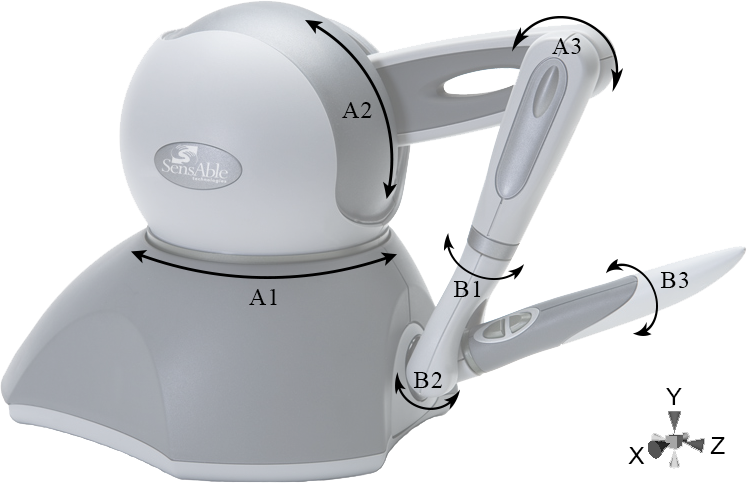
\includegraphics[width=1.0\columnwidth]{figures/omniSchematic.png}
\centering
  \caption{The PHANTOM Omni has six degrees of freedom, three of which provide force feedback (A1-3), and three not providing this feedback; only tracking position (B1-3). \label{fig:omni}}
\end{figure}

\section{Implementation}
The virtual tromba marina consists of several components: visuals, audio, and haptics. 

The application was built using cross-platform game engine Unity \cite{unity}
The raw data provided by the Omni is the following:
\begin{itemize}
    \item absolute position of pivot point B2 (three degrees of freedom)
    \item rotation (three degrees of freedom)
    \item pressure (force depth \textbf{check whether this is correct})
\end{itemize}

The axes are labelled as follows in relation to the virtual instrument: x-axis - width (horizontally across the soundboard -- the common interaction direction), y-axis - height (floor to ceiling) and z-axis - depth (horizontally perpendicular to the soundboard).


The end of the bow -- where a user normally holds it -- has been placed at the pivot point B2 \textbf{$\leftarrow$ not exactly true}
The fact that pivot points B1-3 do not provide force feedback gives rise to an issue in our application. If the virtual
position of pivot point B2 is not the current point of interaction, in the extreme case when the user is bowing using the end of the bow, a force has to be applied as to not go through the string. To solve this issue, we created a separate object with which the bow (pivot point B2 to be exact) will interact with. The y-rotation and y-position of this exactly follows that of the Omni-pen and uses the virtual string as the centerpoint. Furthermore, its position in the x-z--plane is determined by the distance between B2 and the string.

Volume ratios

\subsection{Controls}
As most people are right-handed, it was chosen to also have the bow in the right hand in the application. \textbf{more about bowing hand here}

As the position of the first node along the string is at \begin{equation}\label{eq:node}
    x_\text{node} = L\cdot n^{-1},
\end{equation}
where $L$ is the length of the string and $n = 2,3,...8$ is the harmonic number, we want the damping finger to be set to these positions to induce these harmonics. The lowest harmonic has been set at half the string length $L/2$, i.e., the string is never completely open. The highest harmonic has been chosen to be that can still be played using the model. The location of the damping finger is controlled using the `X' and `Y' buttons and the joystick on the left Oculus controller (see Figure \ref{fig:oculusController}). The buttons are for discrete control of the damping finger, where `Y' increases $n$ in Equation \eqref{eq:node} and `X' decreases it, and the joystick allows for fine pitch control and moves the finger up and down the string. The latter could potentially create pitch glides in the output sound of the application, but make it harder to `hit' a perfect harmonic according to Equation \eqref{eq:node}.

\begin{figure}[ht]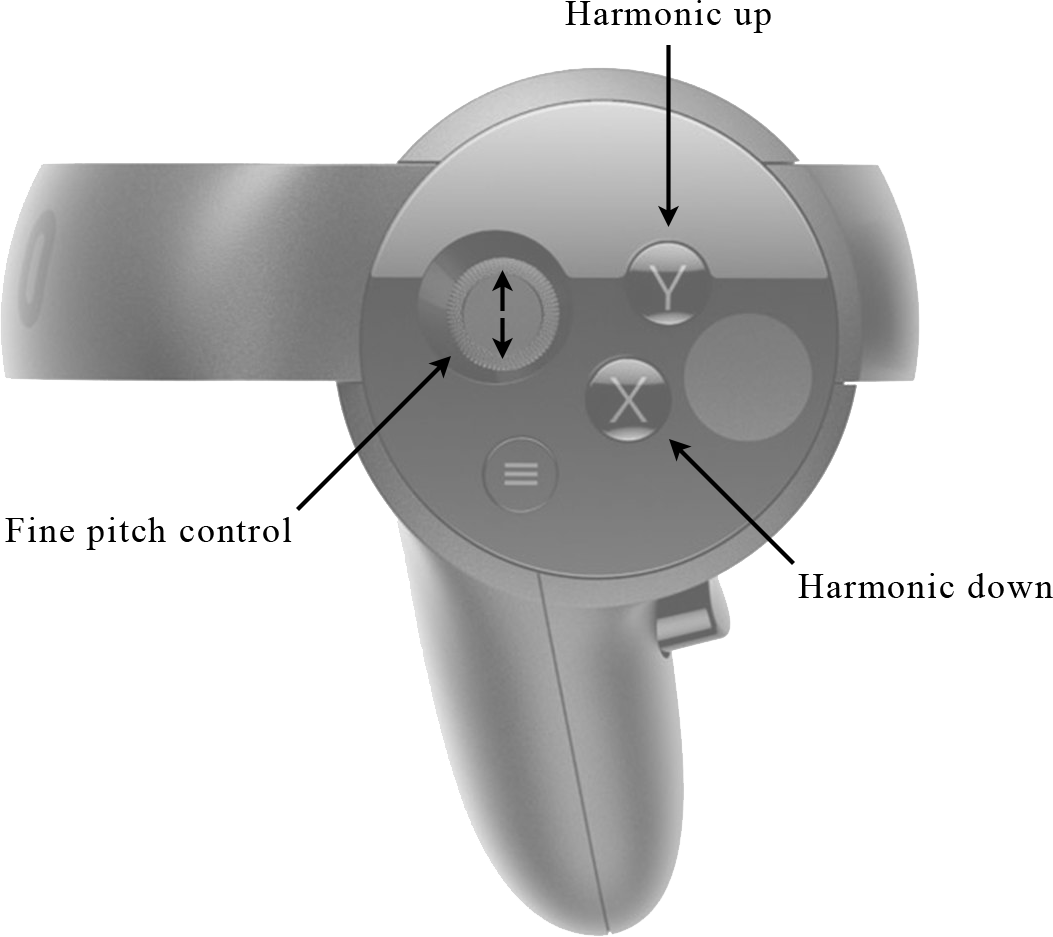
\includegraphics[width=1.0\columnwidth]{SMC 2020 paper template LaTeX/figures/controller.png}
\centering
  \caption{The left Oculus Touch controller. The controls for changing the pitch are highlighted. \label{fig:oculusController}}
\end{figure}

\section{Evaluation}
The evaluation was inspired by \cite{Young2003} \cite{Someren1994} \cite{Stowell2009} and \cite{Finstad2010}


The experiment will be divided in two parts. Firstly, the participants are asked to explore the instrument on their own.

\begin{figure}[ht]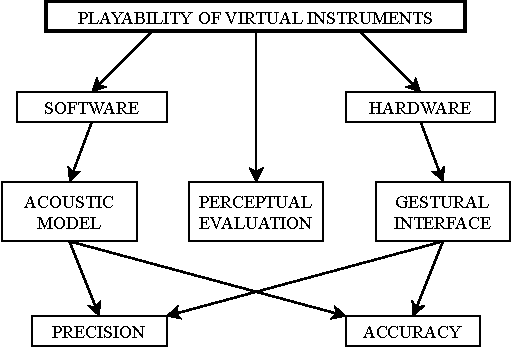
\includegraphics[width=1.0\columnwidth]{SMC 2020 paper template LaTeX/figures/PlayabilityChart.pdf}
\centering
  \caption{Playability chart of a virtual musical instrument \cite{Young2003}. \label{fig:oculusController}}
\end{figure}

\section{Discussion}\label{sec:discussion}
Cognitive load of speech and playing an instrument are ``the same" (Paisa, 2020). So participants speaking their mind while playing might be an issue. Most probably, they will alter between playing and ``thinking aloud". 

\section{Conclusions}
test

\begin{acknowledgments}
Thanks thanksthanks
\end{acknowledgments} 

%%%%%%%%%%%%%%%%%%%%%%%%%%%%%%%%%%%%%%%%%%%%%%%%%%%%%%%%%%%%%%%%%%%%%%%%%%%%%
%bibliography here
\bibliography{smc2020bib}

\end{document}
